\chapter{Lecture 15}

%--- 信息 ----
\begin{center}
    讲师:王立威 \qquad
    课程时间:25.June.3rd \qquad 
    笔记:25.June.9th
\end{center}

\bigskip

(前一部分内容不在考试范围之内,所以等待考试结束后再更新)

现在考虑一个比之前更泛化的最大熵问题 
\begin{example}
    设$X$是一个$d$维的随机变量,满足 
    \[
        \E[X] = \boldsymbol{0}, \quad \cov(X) = \E[XX^\top] = \boldsymbol{\Sigma}
    \]

求最大熵的分布.
\end{example}
\begin{solution}
    我们直接证明最大熵分布是$\cal{N}(\boldsymbol{0}, \boldsymbol{\Sigma})$,取$Y$服从该正态分布,往证明对于任意合意的$X$,都有$h(Y) \ge h(X)$. 

    注意到$D(X\| Y) \ge 0$,而 
    \begin{align*}
        D(X\| Y) & = -h(X) - \int f_X(t) \ln f_Y(t)\dx[t] \\
       & = -h(X) + \frac{1}{2} \ln \left( (2\pi)^d \det \boldsymbol{\Sigma} \right) + \E[X^{\top} \boldsymbol{\Sigma}^{-1} X] \\
        & = -h(X) + \frac{1}{2} \ln \left( (2\pi)^d \det \boldsymbol{\Sigma} \right) + \text{tr}(\boldsymbol{\Sigma}^{-1} \boldsymbol{\Sigma} ) \\
        & = -h(X) + \frac{1}{2} \ln \left( (2\pi)^d \det \boldsymbol{\Sigma} \right) + d \\
        & = -h(X) + h(Y) \ge 0
    \end{align*}

    所以推出$h(Y) \ge h(X)$. 至此证毕.
\end{solution}

\begin{example}
    当$X$是离散型随机变量时,规定取值是$\{0,1,2,\dots\}$,并限定$\E[X] = \mu$. 试求最大熵分布. 
\end{example}
\begin{solution}
    可以算得,最大熵分布是几何分布. 
\end{solution}

% \begin{figure}[H]
%     \centering
%     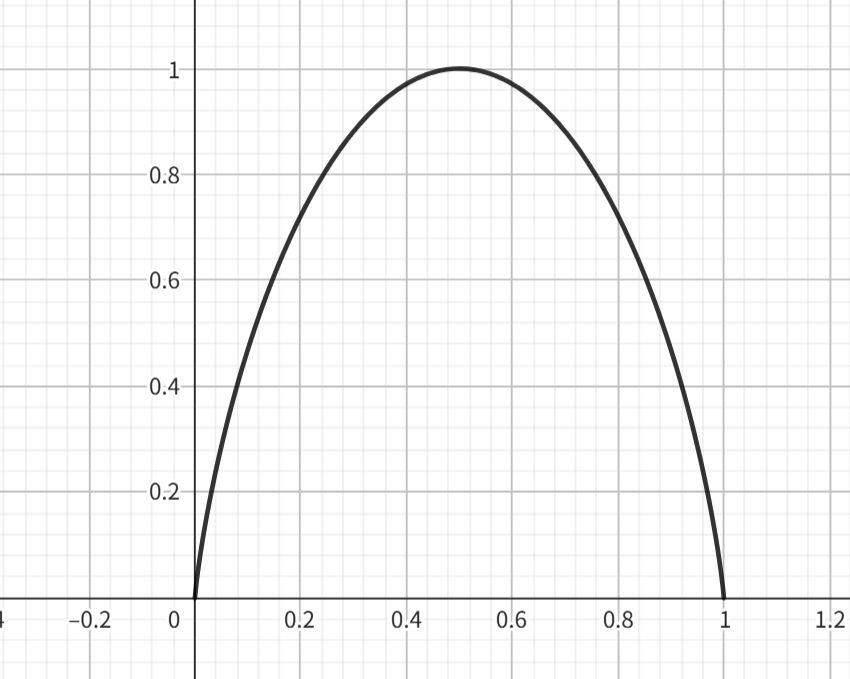
\includegraphics[width=.6\textwidth]{images/c2_1.png}
%     \caption{$H=x\log 1/x + (1-x)\log 1/(1-x)$的图像}
% \end{figure}